\documentclass[10pt,conference,compsocconf]{IEEEtran}

%\usepackage{times}
%\usepackage{balance}
\usepackage{url}
\usepackage{graphicx}
\usepackage{subfigure}	% For figure environment

\begin{document}
\title{Road Segmentation from Satellite Images using\\Support Vector Machine Classification}

\author{
  Daniel Val\'erio Sampaio, Yves Bieri\\
  Department of Computer Science, ETH Zurich, Switzerland
}

\maketitle

\begin{abstract}
	
\end{abstract}

\section{Introduction}

The goal of this paper is to introduce a new road segmentation algorithm for urban areas from satellite images. Road detection is important for several applications from autonomous driving to tracking
of road change and urban planning.

The idea of road segmentation is not a new one and has been implemented numerous times, although with
different success. The great difficulty in urban areas is the occurrence of trees and cars partially blocking the view on roads and thus making detection much harder. Additionally parking lots and railways have a lot of identical features to roads which leads to them being misclassified.

Our approach consists of extracting 16 features from out satellite images and using those to build a Support Vector Machine (SVM) classification model. Our features contain the original image, a smoothed version of said image and a region map, based on a skeletonization approach using an euclidean-like distance map, to reveal the underlying road structure.

The image preprocessing and feature extraction is implemented in \emph{python} with the help of mostly \emph{numpy} and \emph{cv2}. Afterwards the features are fed to MATLAB which is used to produce our SVM classifier. We decided on this approach because \emph{MATLAB} is faster and easier to run on the ETH cluster. The predicted results are then fed again to our \emph{python} program for post-processing and to produce our final results.

In section XXX we describe the idea used in our approach in more detail,
followed by the implementation in section XXX and results in section XXX.
Lastly we conclude the paper with a discussion of our work in section XXX and 
give ideas for future work and improvement.

\section{Models and Methods}
To detect roads from satellite images we decided to use Support Vector Machines (SVM) for classification. We were given 100 training images with corresponding ground truth, which we used to classify 50 test images in a second step.

For the data-driven classifier to be effective, we decided on a set of key features which we extracted from both the training images and the test images. Contrary to our initial implementation, we decided to not consider every single pixel in the image but to form patches instead. We mostly worked with 4x4, 5x5 and 10x10 patches and eventually decided on keeping the 5x5 patching, which offered a good computational speedup without loosing a lot of information of the image features.

The training and test images were taken from urban areas, which apart from roads contain mostly buildings, trees and cars. A road is a long and compared to its length thin object, often in horizontal or vertical direction and colored in a shade of gray. By concentrating on those key characteristics of a road we build a set of features which we will extract to train our model.

The first feature we use is the color in the image patch. It is only natural to include this feature, as a road is usually gray. We can decide whether an image patch is gray by looking at its \emph{RGB} values. They not only help us to find roads that look gray, but also let us recognize different objects in other colors. On one of the images for example there is a pool next to a house, which naturally is blue. Of course, blue objects cannot be roads, and are therefore excluded right from the beginning. In contrast, if the values of red, blue and green all are approximately the same, the resulting color is some kind of gray. So adding the color is a first useful feature to build our model. 

As a second feature we decided to add the standard deviation of the color. We stated earlier, that a pixel is gray, if its three \emph{RGB} values are close. This means that if the standard deviation is small, the red, blue and green values are all close together which is a strong indicator that the pixel is gray. 

After a few trial runs on the training images we noticed that there are a lot of small imperfections which perturb our results. Cars, trees and shadow lead to a pretty big error rate. We concluded that we have to smoothen the images to get rid of this source of noise.

To do that, we used a mean-shift filter, also used in a previous work by Banerjee at al.\cite{BaBuMo12}. This filter allows for edge preserving smoothing of our image, which is essential, considering that roads have distinct borders. For a neighborhood around the pixel the new spatial center and mean color value are calculated and at the end assigned to the pixel. As parameters we used a spatial radius and a color distance of $10$, which seemed to produce reasonably good results in our experiment.

\begin{figure}[t]
	\centering
	\subfigure[original\label{fig:original}]
	{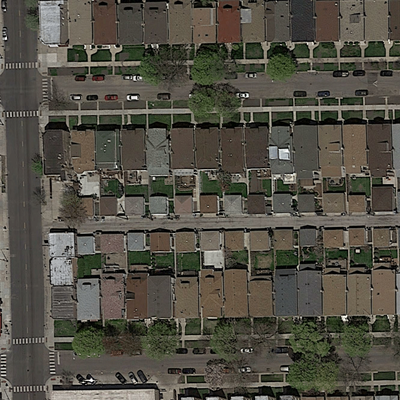
\includegraphics[width=0.49\linewidth]{pics/original.png}}
	\subfigure[mean-shift filtered \label{fig:mean-shift-filtered}]
	{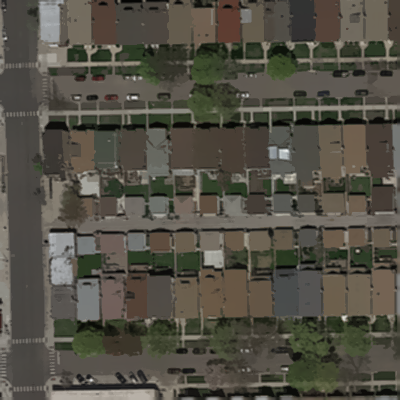
\includegraphics[width=0.49\linewidth]{pics/mean_shifted.png}}
	\caption{Smoothing the original image}
\end{figure}

In addition to the previous mean and standard deviation \emph{RGB} values of the original image, we added the ones obtained by the mean-shift filtered images as our third and fourth parameters of our feature vector. 

We wanted to have the original image but also a smoothed version with less noise. We are convinced that the combination of those two pictures are a good basis for road detection.

Out last, and most complex feature is based on the paper by Gaetano et al. \cite{GaZeScPo11}. The morphological analysis the paper is based on assumes that roads are objects that spread over a rather large part of the image and that have a comparatively small width compared to their total length. Building a morphological skeleton is then the base of the algorithm and consequently for this feature. Ideally a road can afterwards be approximately represented by a branch of the skeleton.

Lets take a look at a brief overview of the algorithm. First edge detection is conducted on the image. The result is then used to compute an euclidean-like distance map (EDM) which then is used to extract the morphological skeleton. Skeletonization although is not very robust, making it therefore desirable to improve it in a post-processing step. To do that, firstly the lines are thinned to a one-pixel width. As we still have too much noise, we also need to remove small branches that are very unlikely to be part of a road. This step is called skeleton pruning. Finally double thresholding is applied to classify valid branches in the skeleton. We consider the average distance in the distance map of every pixel in a skeleton branch and also the overall average distance of every pixel. In the end a watershed transform is applied to reconstruct an image containing various regions, indicating if there is a possible road or not.


So lets look at the single steps a bit more in depth.

1. The first step is edge detection. A python implementation of the canny edge detector is used. Canny edge detection has a relative low computational burden, which is useful as it has to be applied to all three color channels. The edge map from the different channels are merged into one combined edge map. This image is now used as basis for the next step.

2. In the second step we prepare for the skeletonization. Out of the edge map we create a distance map. 
We start out by giving all edge pixels from the canny edge map a distance of 1. Now we consider th 8-neighborhood of each edge pixel. The 8-neighborhood are the 8 pixel that form a 1 pixel wide border around our center pixel. The four horizontal and vertical neighbors are given a distance of +1. Meaning that if the center pixel had distance 1, they get assigned distance 2. For the four diagonal pixels we add $\sqrt{2}$ to the value of the center pixel. By assigning a higher value to the diagonal pixels we generate smoother curves and more exact distance values for further computations. We continue those steps iteratively until all pixels are assigned a value. From now on we refer to the result of this step as the euclidean distance map (EDM).

3. Now, in the third step, we create the skeleton out of our EDM. For this we use a crest line following approach descriped in paper XXX. With the crest line approach we want to find a relatively simple skeleton. One single straight line is enough to represent a road pretty accurately. As in the urban are most roads are either horizontal or vertical without curves this approach gives us a pretty good result. 

Now we look at all the points from the EDM which have a maximum of two neighbors with higher value ar considered crest line points. With this approach we recursively add the neighboring points with the steepest ascent to our crest line. Finally we apply morphological thinning to reduce our crest lines to 1 pixel in width.

4. The forth step consists of pruning the skeleton. The road skeleton obtained in step 3 has a lot of small branches that are most likely not part of a road and thus generate noise. By pruning the skeleton we can enhance the representation of our roads. In our skeleton map we mark all leave nodes yellow and all intersection nodes green. Afterwards we consider all nodes with connection degree of one or lower. And remove those nodes together with the edge/branch between this node and the one on the other side of the edge. This eliminates a lot of small noisy branches. 


5. Now in the final step we do road detection and map reconstruction. For this we use a double thresholding method. Recall that we can describe a road as a branch of the skeleton with a large length compared to its width. The first value we threshold is the average distance of a skeleton segment divided by its length. This measure is called the road skeleton score (RSS). In the paper the propose to set $RSS_th = 0.04$. The second threshold $D_th$ is set to $12$. This is the average distance function over the skeleton points and calculated as ${D_i}_avg = sum(p \in S_i) * D(p) / |S_i|$. We keep all the pixels that are smaller than both those thresholds. 

Lastly we apply a marker based watershed transform on the distance function to reconstruct our map. The watershed transformation summarizes large similar patches and we color them with the mean color of the original image in that region. We obtain a segmentation map where each connected component contains exactly one connected skeleton segment. 



\begin{enumerate}
\item Layout the model you used to describe the problem or the solution.
\item Describing the algorithms used in the study, briefly including
  details such as hyperparameter values (e.g. thresholds), and
  preprocessing steps (e.g. normalizing the data to have mean value of
  zero).
\item Explaining how the materials were prepared, for example the
  images used and their resolution.
\item Describing the research protocol, for example which examples
  were used for estimating the parameters (training) and which were
  used for computing performance.
\item Explaining how measurements were made and what
  calculations were performed. Do not reproduce the full source code in
  the paper, but explain the key steps.
\end{enumerate}

\subsection{Results}

Organize the results section based on the sequence of table and
figures you include. Prepare the tables and figures as soon as all
the data are analyzed and arrange them in the sequence that best
presents your findings in a logical way. A good strategy is to note,
on a draft of each table or figure, the one or two key results you
want to address in the text portion of the results.
The information from the figures is
summarized in Table~\ref{tab:fourier-wavelet}.

\begin{table*}[htbp]
  \centering
  \begin{tabular}[c]{|l||l|l|l|}
    \hline
    Basis&Support&Suitable signals&Unsuitable signals\\
    \hline
    Fourier&global&sine like&localized\\
    wavelet&local&localized&sine like\\
    \hline
  \end{tabular}
  \caption{Characteristics of Fourier and wavelet basis.}
  \label{tab:fourier-wavelet}
\end{table*}

When reporting computational or measurement results, always
report the mean (average value) along with a measure of variability
(standard deviation(s) or standard error of the mean).


\section{Tips for Good Software}
\label{sec:tips-software}

There is a lot of literature (for example~\cite{hunt99pragmatic} and
\cite{spolsky04software}) on how to write software. It is not the
intention of this section to replace software engineering
courses. However, in the interests of reproducible
research~\cite{schwab00}, there are a few guidelines to make your
reader happy:
\begin{itemize}
\item Have a \texttt{README} file that (at least) describes what your
  software does, and which commands to run to obtain results. Also
  mention anything special that needs to be set up, such as
  toolboxes\footnote{For those who are
  particularly interested, other common structures can be found at
  \url{http://en.wikipedia.org/wiki/README} and
  \url{http://www.gnu.org/software/womb/gnits/}.}.
\item A list of authors and contributors can be included in a file
  called \texttt{AUTHORS}, acknowledging any help that you may have
  obtained. For small projects, this information is often also
  included in the \texttt{README}.
\item Use meaningful filenames, and not \texttt{temp1.m},
  \texttt{temp2.m}. The code should also unzip into a subdirectory.
\item Document your code. Each file should at least have a short
  description about its reason for existence. Non obvious steps in the
  code should be commented.
\item Describe how the results presented in your paper can potentially
  be reproduced.
\end{itemize}


\section{Computational Intelligence Laboratory Requirements}
\label{sec:cil}

Your semester project is a group effort. It consists of four parts:
\begin{enumerate}
\item The programming assignments you solve during the semester.
\item Developing a novel solution for one of the assignments, e.g. by
  combining methods from previous programming assignments into a novel
  solution.
\item Comparing your novel solution to previous assignments.
\item Writing up your findings in a short scientific paper.
\end{enumerate}

\subsection{Developing a Novel Solution}

As your final programming assignment, you develop a novel solution to
one of the four application problems. You are free to exploit any idea
you have, provided it is not identical to any other group submission
or existing Matlab implementation of an algorithm on the
internet\footnote{\url{http://www.ethz.ch/students/semester/plagiarism_s_en.pdf}}.

Two examples for developing a novel solution:
\begin{itemize}
\item You implemented a collaborative filtering algorithm based on
  dimension reduction as part of an assignment. Now you apply
  dimension reduction to inpainting.
\item You implemented both a clustering and a sparse coding algorithm
  for image compression. Now you combine both techniques into a novel
  compression method.
\end{itemize}

\subsection{Comparison to Baselines}

You compare your novel algorithm to \emph{at least two baseline
  algorithms}. For the baselines, you can use the implementations you
developed as part of the programming assignments.


\subsection{Write Up}

The submission must be in PDF form, using the \LaTeX{} template
corresponding to the IEEE style of publication. Refer to
Section~\ref{sec:latex-primer} for more information about preparing
your document. The document should be a maximum of {\bf 4 pages}.

\subsection{\LaTeX{} Primer}
\label{sec:latex-primer}

\LaTeX{} is one of the most commonly used document preparation systems
for scientific journals and conferences. It is based on the idea
that authors should be able to focus on the content of what they are
writing without being distracted by its visual presentation.
The source of this file can be used as a starting point for how to use
the different commands in \LaTeX{}. We are using an IEEE style for
this course.

\subsubsection{Installation}

There are various different packages available for processing \LaTeX{}
documents.
On Windows, use the Mik\TeX{} package (\url{http://miktex.org/}), and
on OSX use MacTeX
(\url{http://www.tug.org/mactex/2009/}). Alternatively, on OSX, you
can install the \texttt{tetex} package via
Fink\footnote{\url{http://www.finkproject.org/}} or 
Macports\footnote{\url{http://www.macports.org/}}.

\subsubsection{Compiling \LaTeX{}}
Your directory should contain at least 4 files, in addition to image
files. Images should be in \texttt{.png}, \texttt{.jpg} or
\texttt{.pdf} format.
\begin{itemize}
\item IEEEtran.cls
\item IEEEtran.bst
\item groupXX-submission.tex
\item groupXX-literature.bib
\end{itemize}
Note that you should replace groupXX with your chosen group name.
Then, from the command line, type:
\begin{verbatim}
$ pdflatex groupXX-submission
$ bibtex groupXX-literature
$ pdflatex groupXX-submission
$ pdflatex groupXX-submission
\end{verbatim}
This should give you a PDF document \texttt{groupXX-submission.pdf}.

\subsubsection{Equations}

There are three types of equations available: inline equations, for
example $y=mx + c$, which appear in the text, unnumbered equations
$$y=mx + c,$$
which are presented on a line on its own, and numbered equations
\begin{equation}
  \label{eq:linear}
  y = mx + c
\end{equation}
which you can refer to at a later point (Equation~(\ref{eq:linear})).

\subsubsection{Tables and Figures}

Tables and figures are ``floating'' objects, which means that the text
can flow around it.
Note
that \texttt{figure*} and \texttt{table*} cause the corresponding
figure or table to span both columns.


\subsection{Grading}

There are two different types of grading criteria applied to your
project, with the corresponding weights shown in brackets.
\begin{description}
\item[Competitive] \ \\
  The following criteria is scored based on your rank
  in comparison with the rest of the class.
  \begin{itemize}
  \item time taken for computation (10\%)
  \item average rank for all other criteria relevant to the task, for
    example reconstruction error and sparsity (20\%)
  \end{itemize}
  The ranks will then be converted on a linear scale into a grade
  between 4 and 6.
\item[Non-competitive] \ \\
  The following criteria is scored based on an
  evaluation by the teaching assistants.
  \begin{itemize}
  \item quality of paper (30\%)
  \item quality of implementation (20\%)
  \item creativity of solution (20\%)
  \end{itemize}
\end{description}

\subsection{Submission System}

The deadline for submitting your project report is Friday, 22 June
2012.
You need to submit:
\begin{itemize}
\item PDF of paper.
\item Archive (\texttt{.tar.gz} or \texttt{.zip}) of software. Please
  do not forget to include author information in the source archive.
\end{itemize}

\textbf{Important:} Please check the submission instructions on the webpage 
as it is the most updated instructions. 

\section{Summary}

The aim of a scientific paper is to convey the idea or discovery of
the researcher to the minds of the readers. The associated software
package provides the relevant details, which are often only briefly
explained in the paper, such that the research can be reproduced.
To write good papers, identify your key idea, make your contributions
explicit, and use examples and illustrations to describe the problems
and solutions.

\section*{Acknowledgements}
The author thanks Christian Sigg for his careful reading and helpful
suggestions.

\bibliographystyle{IEEEtran}
\bibliography{howto-paper}
\end{document}
